% Options for packages loaded elsewhere
\PassOptionsToPackage{unicode}{hyperref}
\PassOptionsToPackage{hyphens}{url}
\PassOptionsToPackage{dvipsnames,svgnames,x11names}{xcolor}
\documentclass[
]{article}
\usepackage{xcolor}
\usepackage[margin=1in]{geometry}
\usepackage{amsmath,amssymb}
\setcounter{secnumdepth}{-\maxdimen} % remove section numbering
\usepackage{iftex}
\ifPDFTeX
  \usepackage[T1]{fontenc}
  \usepackage[utf8]{inputenc}
  \usepackage{textcomp} % provide euro and other symbols
\else % if luatex or xetex
  \usepackage{unicode-math} % this also loads fontspec
  \defaultfontfeatures{Scale=MatchLowercase}
  \defaultfontfeatures[\rmfamily]{Ligatures=TeX,Scale=1}
\fi
\usepackage{lmodern}
\ifPDFTeX\else
  % xetex/luatex font selection
\fi
% Use upquote if available, for straight quotes in verbatim environments
\IfFileExists{upquote.sty}{\usepackage{upquote}}{}
\IfFileExists{microtype.sty}{% use microtype if available
  \usepackage[]{microtype}
  \UseMicrotypeSet[protrusion]{basicmath} % disable protrusion for tt fonts
}{}
\makeatletter
\@ifundefined{KOMAClassName}{% if non-KOMA class
  \IfFileExists{parskip.sty}{%
    \usepackage{parskip}
  }{% else
    \setlength{\parindent}{0pt}
    \setlength{\parskip}{6pt plus 2pt minus 1pt}}
}{% if KOMA class
  \KOMAoptions{parskip=half}}
\makeatother
\usepackage{longtable,booktabs,array}
\usepackage{calc} % for calculating minipage widths
% Correct order of tables after \paragraph or \subparagraph
\usepackage{etoolbox}
\makeatletter
\patchcmd\longtable{\par}{\if@noskipsec\mbox{}\fi\par}{}{}
\makeatother
% Allow footnotes in longtable head/foot
\IfFileExists{footnotehyper.sty}{\usepackage{footnotehyper}}{\usepackage{footnote}}
\makesavenoteenv{longtable}
\usepackage{graphicx}
\makeatletter
\newsavebox\pandoc@box
\newcommand*\pandocbounded[1]{% scales image to fit in text height/width
  \sbox\pandoc@box{#1}%
  \Gscale@div\@tempa{\textheight}{\dimexpr\ht\pandoc@box+\dp\pandoc@box\relax}%
  \Gscale@div\@tempb{\linewidth}{\wd\pandoc@box}%
  \ifdim\@tempb\p@<\@tempa\p@\let\@tempa\@tempb\fi% select the smaller of both
  \ifdim\@tempa\p@<\p@\scalebox{\@tempa}{\usebox\pandoc@box}%
  \else\usebox{\pandoc@box}%
  \fi%
}
% Set default figure placement to htbp
\def\fps@figure{htbp}
\makeatother
% definitions for citeproc citations
\NewDocumentCommand\citeproctext{}{}
\NewDocumentCommand\citeproc{mm}{%
  \begingroup\def\citeproctext{#2}\cite{#1}\endgroup}
\makeatletter
 % allow citations to break across lines
 \let\@cite@ofmt\@firstofone
 % avoid brackets around text for \cite:
 \def\@biblabel#1{}
 \def\@cite#1#2{{#1\if@tempswa , #2\fi}}
\makeatother
\newlength{\cslhangindent}
\setlength{\cslhangindent}{1.5em}
\newlength{\csllabelwidth}
\setlength{\csllabelwidth}{3em}
\newenvironment{CSLReferences}[2] % #1 hanging-indent, #2 entry-spacing
 {\begin{list}{}{%
  \setlength{\itemindent}{0pt}
  \setlength{\leftmargin}{0pt}
  \setlength{\parsep}{0pt}
  % turn on hanging indent if param 1 is 1
  \ifodd #1
   \setlength{\leftmargin}{\cslhangindent}
   \setlength{\itemindent}{-1\cslhangindent}
  \fi
  % set entry spacing
  \setlength{\itemsep}{#2\baselineskip}}}
 {\end{list}}
\usepackage{calc}
\newcommand{\CSLBlock}[1]{\hfill\break\parbox[t]{\linewidth}{\strut\ignorespaces#1\strut}}
\newcommand{\CSLLeftMargin}[1]{\parbox[t]{\csllabelwidth}{\strut#1\strut}}
\newcommand{\CSLRightInline}[1]{\parbox[t]{\linewidth - \csllabelwidth}{\strut#1\strut}}
\newcommand{\CSLIndent}[1]{\hspace{\cslhangindent}#1}
\setlength{\emergencystretch}{3em} % prevent overfull lines
\providecommand{\tightlist}{%
  \setlength{\itemsep}{0pt}\setlength{\parskip}{0pt}}
% Set up the fonts
\usepackage[urw-palatino]{mathdesign}
\usepackage[T1]{fontenc}


% Set the language for 508
\usepackage{hyperref}
\hypersetup{
  pdftitle = {title},
  pdflang = en-US}

% Add accessibility support from http://www.richschwinn.com/accessibility
\RequirePackage{accsupp}
\RequirePackage{pdfcomment}
\newcommand{\AccTool}[2]{\BeginAccSupp{method=pdfstringdef,unicode,Alt={{#1}}}\pdftooltip{{#2}}{{#1}}\EndAccSupp{}}


% Set up the headers and footers
\usepackage{graphicx}
\usepackage{fancyhdr}
\usepackage{ifthen}
%\usepackage{everypage-1x}
\usepackage{float}
%\usepackage{subfig}
%\usepackage{subcaption}

% Avoid struggling over figure and table float in Rmarkdown
\let\origfigure\figure
\let\endorigfigure\endfigure
\renewenvironment{figure}[1][2] {
    \expandafter\origfigure\expandafter[H]
} {
    \endorigfigure
}

\let\origtable\table
\let\endorigtable\endtable
\renewenvironment{table}[1][2] {
    \expandafter\origtable\expandafter[H]
} {
    \endorigtable
}

% First page has the large title and NOAA logo
%\pagestyle{fancy}
%\fancyhf{}
%\setlength\headheight{40pt}
%\fancyheadoffset[L]{0.5cm}
%\cfoot{\thepage}
%
%\fancyheadinit{%
%   \ifthenelse{\value{page}=4}%
%      {\fancyhead[R]{\includegraphics[width=40pt]{images/NOAA_logo.png} \\ \textsf{\emph{March 17, 2022}}}
%       \fancyhead[L]{\textsf{\LARGE State of the Ecosystem 2022: Mid-Atlantic}}
%      }%
%      {\fancyhead[R]{}
%       \fancyhead[L]{\textsf{\emph{State of the Ecosystem 2022: Mid-Atlantic}}}
%      }
%}



\renewcommand{\headrulewidth}{0.4pt}
\renewcommand{\footrulewidth}{0pt}

% Make caption fonts a bit smaller
\usepackage[font={small}]{caption}


% Change section labels to san serif
\usepackage{sectsty}
\allsectionsfont{\normalfont\sffamily\bfseries}

%\usepackage{lineno}
%\linenumbers

%\usepackage{setspace}
%\doublespacing
\usepackage{multirow}
\usepackage{multicol}
\usepackage{colortbl}
\usepackage{hhline}
\newlength\Oldarrayrulewidth
\newlength\Oldtabcolsep
\usepackage{longtable}
\usepackage{array}
\usepackage{hyperref}
\usepackage{float}
\usepackage{wrapfig}
\usepackage{bookmark}
\IfFileExists{xurl.sty}{\usepackage{xurl}}{} % add URL line breaks if available
\urlstyle{same}
\hypersetup{
  pdftitle={MAFMC Indicators Project Online Mini Workshop Report},
  pdfauthor={Sarah Gaichas, Kelsey Roberts, Gavin Fay, Sophie Wulfing},
  colorlinks=true,
  linkcolor={Maroon},
  filecolor={Maroon},
  citecolor={Blue},
  urlcolor={blue},
  pdfcreator={LaTeX via pandoc}}

\title{MAFMC Indicators Project Online Mini Workshop Report}
\author{Sarah Gaichas, Kelsey Roberts, Gavin Fay, Sophie Wulfing}
\date{2026-05-05}

\begin{document}
\maketitle

\section{Executive Summary}\label{executive-summary}

The Mid-Atlantic Fishery Management Council Inflation Reduction Act Project 5, ``Operationalizing Ecosystem and Habitat Indicators to Support Climate-Ready Fisheries Management in the Mid-Atlantic'' (MAFMC Indicators Project) held an online workshop on March 31, 2026. The workshop focused on transitioning from the broader review phase of the project to phase two developing and testing specific indicators for decision-making. The workshop objective was to outline development of indicators and processes to use them in 2 priority Council management decisions. Workshop materials are posted at \url{https://www.mafmc.org/council-events/2026/eco-hab-indicators-workshop}.

A total of 33 people attended the workshop, including 28 participants from the Council, Council Advisory Panels, Scientific and Statistical Committee (SSC), Council staff, as well as staff from the New England Council, Atlantic States Marine Fisheries Commission, Greater Atlantic Regional Fisheries Office, and the Northeast Fisheries Science Center, in addition to the project team. Five University of Massachusetts School for Marine Science and Technology graduate students also attended and supported the meeting.

The 2 priority management decisions were selected from the list of 4 decisions developed in \href{https://www.mafmc.org/council-events/2025/dec-10/indicators-workshop}{December 2025} based on responses to polling conducted prior to the online workshop and confirmed by workshop participants. Selected decisions were:

\begin{enumerate}
\def\labelenumi{\arabic{enumi}.}
\tightlist
\item
  \href{https://www.mafmc.org/s/3_MiniWK_RiskPolicy.pdf}{Risk Policy}
\item
  \href{https://www.mafmc.org/s/4_MiniWK_CatchQuotas.pdf}{Catch/Quota Setting}
\end{enumerate}

The workshop included an introductory presentation from the project team, including poll results, followed by three discussions to scope development of operational ecosystem indicators for the 2 priority decisions. Discussion 1 reviewed the relative merits of developing indicators for each priority decision. Discussion 2 identified desirable and undesirable states for management outcomes. Discussion 3 outlined potential indicator targets or thresholds tied to desirable and undesirable states. The key takeaways of each discussion are outlined here.

\subsection{Discussion 1: Indicators and approach for each decision}\label{discussion-1-indicators-and-approach-for-each-decision}

\begin{itemize}
\tightlist
\item
  \textbf{Risk policy:} consider social or economic risk indicators in addition to stock status while retaining overall simplicity of the approach and consistent application across species. Start by reviewing cases where the Council has suspended the risk policy. Retain broad scope for application across species.
\item
  \textbf{Catch/quota setting:} review and communicate ecosystem/habitat information available/used throughout the process to ensure indicators are not ``double counted''. Consider information used in prioritization and assessment but focus on developing new indicators for SSC ABC, Monitoring Committee, and Council processes. Consider a detailed application for a particular species.
\end{itemize}

\subsection{Discussion 2: Desirable and undesirable states}\label{discussion-2-desirable-and-undesirable-states}

\begin{itemize}
\tightlist
\item
  \textbf{Desirable:} transparent and relatively simple decision processes, decisions reflect reality, interannual stability, ability to assess tradeoffs across objectives
\item
  \textbf{Undesirable:} overly complex processes, cascading unforeseen impacts of decisions resulting in reactive rather than proactive management, large interannual swings in management outcomes, accounting for conditions in more than one place (double counting)
\end{itemize}

\subsection{Discussion 3: Targets and thresholds}\label{discussion-3-targets-and-thresholds}

\begin{itemize}
\tightlist
\item
  \textbf{Characteristics:} targets as ranges rather than points, surveillance indicators to determine if conditions leave target range, historical baselines could provide initial target ranges but recognize and adapt to changing conditions, apply targets similarly across fishery sectors
\item
  \textbf{Other considerations:} indicators that imply certainty or reduce uncertainty are desirable
\end{itemize}

The next steps for the project are:

\begin{enumerate}
\def\labelenumi{\arabic{enumi}.}
\tightlist
\item
  to evaluate information sources and develop indicators that address the priority management decisions,
\item
  to evaluate theoretical and empirical thresholds for the indicators relating to the management decisions
\item
  to develop and apply frameworks to test the use of indicators in each decision, and
\item
  to prepare interim results for a workshop outlining performance metrics in late 2026.
\end{enumerate}

\section{Introduction}\label{introduction}

The Mid-Atlantic Fishery Management Council Inflation Reduction Act Project 5, ``Operationalizing Ecosystem and Habitat Indicators to Support Climate-Ready Fisheries Management in the Mid-Atlantic'' (MAFMC Indicators Project) has been designed to address the Council's April 2025 request to

\begin{quote}
``(1) conduct a comprehensive review of ecosystem and habitat indicators that will support management objectives, and (2) identify management processes, documents, and/or actions where ecosystem and habitat indicators can be integrated to inform management decisions.''
\end{quote}

The MAFMC Indicators Project addresses three Council objectives:

\begin{enumerate}
\def\labelenumi{\arabic{enumi}.}
\tightlist
\item
  Review and assess existing ecosystem and habitat indicators in the Northeast and evaluate their utility to support management objectives.
\item
  Identify and develop priority ecosystem and habitat indicators, including associated targets and thresholds as appropriate, and identify specific pathways for incorporation into Council management processes, documents, or actions.
\item
  Create workflow and communication tools to support regular updates of indicators and that enhance usability of indicators in the management process.
\end{enumerate}

To address these objectives, the project team continues to conduct a comprehensive review of existing indicators, has developed a framework for evaluating the indicators, and organized an initial workshop in December 2025 to identify and prioritize Council management decisions that could be supported or improved by operational use of ecosystem indicators. The \href{https://www.mafmc.org/s/WK1_Report.pdf}{Workshop 1 Report} and \href{https://www.mafmc.org/s/WK1_Results-Summary.pdf}{Workshop 1 Outcomes Summary} summarized the presentations, discussions, and outcomes of Workshop 1.

Four management decisions were identified at Workshop 1: Risk Policy, Catch/Quota Setting, Measures Setting, and Spatial Management. After Workshop 1, the project team outlined the current decision processes and information used for each of the four decisions, and identified potential information sources for new indicators and pathways to use new indicators in each decision. This information was summarized in a series of short, decision-specific 1 page reports that were provided to workshop participants in advance of the online mini-workshop, which is the subject of this report.

While the online mini-workshop was a public meeting open to all interested participants, some Council, Advisory Panel, Scientific and Statistical Committee (SSC), and Atlantic States Marine Fisheries Commission (ASMFC) and Council staff members that participated in the December 2025 workshop were specifically invited to participate based on their prior experience with the project and with Council ecosystem and habitat indicators, and to encourage participation across a range of stakeholder groups.

A brief online poll (described below) and all of the short reports were distributed to invited participants the week prior to the workshop to solicit priorities for project focus from as many individuals as possible.

The workshop was held online March 31, 2026. Workshop materials are posted at \url{https://www.mafmc.org/council-events/2026/eco-hab-indicators-workshop}.

The workshop was well-attended. A total of 33 people attended the workshop. Attendees included 28 participants from the Council, Council Advisory Panels, SSC, Council staff, as well as staff from the New England Council, ASMFC, Greater Atlantic Regional Fisheries Office (GARFO), and the Northeast Fisheries Science Center (NEFSC), in addition to the project team. Five graduate students from the University of Massachusetts Dartmouth School for Marine Science and Technology also attended and supported the meeting.

The workshop agenda is included as Appendix 1 and the list of attendees is included as Appendix 2. The remaining workshop materials are included as Appendices 3-11. The presentation shown during the workshop is linked below.

A 1-page workshop summary was also developed and is included as Appendix 12.

\section{Workshop Presentation Summary}\label{workshop-presentation-summary}

The workshop began with a round of introductions, followed by an introductory presentation. The \href{https://sgaichas.github.io/HSpresentations/20260331_ProjectOverview_MiniWK_Gaichas.html}{presentation} briefly reviewed the overall MAFMC Indicators Project goals and objectives, timeline, current progress, and planned activities.

\subsection{Pre-workshop Poll Results}\label{pre-workshop-poll-results}

Poll results were then summarized. The poll had four multiple choice questions and two short answer questions:

\begin{enumerate}
\def\labelenumi{\arabic{enumi}.}
\tightlist
\item
  What is the highest priority management measure this project should focus on?

  \begin{itemize}
  \tightlist
  \item
    Risk Policy
  \item
    Catch/Quota Setting
  \item
    Measures Setting
  \item
    Spatial Measures
  \end{itemize}
\item
  What is the scope of the highest priority management decision that this project should focus on?

  \begin{itemize}
  \tightlist
  \item
    Develop a general process that could work across species/FMPs
  \item
    Develop a detailed example tailored to a particular species (Please write in species below)
  \end{itemize}
\item
  If a detailed example is preferred, which species should be the focus?

  \begin{itemize}
  \tightlist
  \item
    {[}short answer{]}
  \end{itemize}
\item
  What is the next highest priority management measure this project should focus on?

  \begin{itemize}
  \tightlist
  \item
    Risk Policy
  \item
    Catch/Quota Setting
  \item
    Measures Setting
  \item
    Spatial Measures
  \end{itemize}
\item
  What is the scope of the next highest priority management decision that this project should focus on?

  \begin{itemize}
  \tightlist
  \item
    Develop a general process that could work across species/FMPs
  \item
    Develop a detailed example tailored to a particular species (Please write in species below)
  \end{itemize}
\item
  If a detailed example is preferred, which species should be the focus?

  \begin{itemize}
  \tightlist
  \item
    {[}short answer{]}
  \end{itemize}
\end{enumerate}

Results for each question showed a majority prioritizing Risk Policy first. The next highest priority decision measured across all respondents was Catch/Quota setting (Fig. \ref{fig:priority1}, Table \ref{tab:poll}).

\begin{figure}

{\centering \includegraphics[width=0.8\linewidth]{MiniWK_Report_files/figure-latex/priority1-1} 

}

\caption{Pre-workshop poll results}\label{fig:priority1}
\end{figure}

\global\setlength{\Oldarrayrulewidth}{\arrayrulewidth}

\global\setlength{\Oldtabcolsep}{\tabcolsep}

\setlength{\tabcolsep}{2pt}

\renewcommand*{\arraystretch}{1.2}



\providecommand{\ascline}[3]{\noalign{\global\arrayrulewidth #1}\arrayrulecolor[HTML]{#2}\cline{#3}}

\begin{longtable}[c]{|p{2.00in}|p{1.00in}|p{1.00in}}

\caption{Summary\ poll\ results\ across\ both\ questions}\label{tab:poll}\\

\ascline{1.5pt}{666666}{1-3}

\multicolumn{1}{>{\raggedright}m{\dimexpr 2in+0\tabcolsep}}{\textcolor[HTML]{000000}{\fontsize{11}{11}\selectfont{Decision}}} & \multicolumn{1}{>{\raggedleft}m{\dimexpr 1in+0\tabcolsep}}{\textcolor[HTML]{000000}{\fontsize{11}{11}\selectfont{Votes}}} & \multicolumn{1}{>{\raggedleft}m{\dimexpr 1in+0\tabcolsep}}{\textcolor[HTML]{000000}{\fontsize{11}{11}\selectfont{\%\ Total\ Votes}}} \\

\ascline{1.5pt}{666666}{1-3}\endfirsthead \caption[]{Summary\ poll\ results\ across\ both\ questions}\label{tab:poll}\\

\ascline{1.5pt}{666666}{1-3}

\multicolumn{1}{>{\raggedright}m{\dimexpr 2in+0\tabcolsep}}{\textcolor[HTML]{000000}{\fontsize{11}{11}\selectfont{Decision}}} & \multicolumn{1}{>{\raggedleft}m{\dimexpr 1in+0\tabcolsep}}{\textcolor[HTML]{000000}{\fontsize{11}{11}\selectfont{Votes}}} & \multicolumn{1}{>{\raggedleft}m{\dimexpr 1in+0\tabcolsep}}{\textcolor[HTML]{000000}{\fontsize{11}{11}\selectfont{\%\ Total\ Votes}}} \\

\ascline{1.5pt}{666666}{1-3}\endhead



\multicolumn{1}{>{\raggedright}m{\dimexpr 2in+0\tabcolsep}}{\textcolor[HTML]{000000}{\fontsize{11}{11}\selectfont{Risk\ Policy}}} & \multicolumn{1}{>{\raggedleft}m{\dimexpr 1in+0\tabcolsep}}{\textcolor[HTML]{000000}{\fontsize{11}{11}\selectfont{8}}} & \multicolumn{1}{>{\raggedleft}m{\dimexpr 1in+0\tabcolsep}}{\textcolor[HTML]{000000}{\fontsize{11}{11}\selectfont{67}}} \\





\multicolumn{1}{>{\raggedright}m{\dimexpr 2in+0\tabcolsep}}{\textcolor[HTML]{000000}{\fontsize{11}{11}\selectfont{Catch/Quota\ Setting}}} & \multicolumn{1}{>{\raggedleft}m{\dimexpr 1in+0\tabcolsep}}{\textcolor[HTML]{000000}{\fontsize{11}{11}\selectfont{7}}} & \multicolumn{1}{>{\raggedleft}m{\dimexpr 1in+0\tabcolsep}}{\textcolor[HTML]{000000}{\fontsize{11}{11}\selectfont{58}}} \\





\multicolumn{1}{>{\raggedright}m{\dimexpr 2in+0\tabcolsep}}{\textcolor[HTML]{000000}{\fontsize{11}{11}\selectfont{Spatial\ Measures}}} & \multicolumn{1}{>{\raggedleft}m{\dimexpr 1in+0\tabcolsep}}{\textcolor[HTML]{000000}{\fontsize{11}{11}\selectfont{5}}} & \multicolumn{1}{>{\raggedleft}m{\dimexpr 1in+0\tabcolsep}}{\textcolor[HTML]{000000}{\fontsize{11}{11}\selectfont{42}}} \\





\multicolumn{1}{>{\raggedright}m{\dimexpr 2in+0\tabcolsep}}{\textcolor[HTML]{000000}{\fontsize{11}{11}\selectfont{Measures\ Setting}}} & \multicolumn{1}{>{\raggedleft}m{\dimexpr 1in+0\tabcolsep}}{\textcolor[HTML]{000000}{\fontsize{11}{11}\selectfont{4}}} & \multicolumn{1}{>{\raggedleft}m{\dimexpr 1in+0\tabcolsep}}{\textcolor[HTML]{000000}{\fontsize{11}{11}\selectfont{33}}} \\

\ascline{1.5pt}{666666}{1-3}



\end{longtable}



\arrayrulecolor[HTML]{000000}

\global\setlength{\arrayrulewidth}{\Oldarrayrulewidth}

\global\setlength{\tabcolsep}{\Oldtabcolsep}

\renewcommand*{\arraystretch}{1}

(One response received after the workshop selected Catch/Quota setting as highest priority and Measures Setting as the next highest priority.)

All respondents who prioritized ``Risk Policy'' recommended focus on ``General'' scope. ``Catch/Quota Setting'' had 57\% recommending a ``Detailed example'' for one species. However, there was not a clear majority for which species. Summer flounder and black sea bass had the most support considering both the poll and the workshop discussion, but squids were mentioned many times as well.

Next, current processes for each priority decision were reviewed, along with potential information sources and pathways to test and use the indicators.

\subsection{Risk Policy}\label{risk-policy}

Risk policy is a Council-level decision and specifies the Council's risk tolerance (e.g., probability of overfishing) for its managed stocks. Current \href{https://www.federalregister.gov/documents/2020/12/15/2020-27562/fisheries-of-the-northeastern-united-states-omnibus-framework-adjustment-to-modify-the-mid-atlantic}{Risk Policy} uses stock status as the only indicator of when to adjust risk tolerance. Low stock status (B/Bmsy \textless{} 1) results in much more risk averse probability of overfishing and lower ABC relative to OFL. High stock status (\textgreater1.5 B/Bmsy) is nearly as risk tolerant as allowed by law with ABC close to OFL.

\subsubsection{What information is used now?}\label{what-information-is-used-now}

The current Risk Policy (Fig. \ref{fig:MAFMCriskpolicy}) was finalized by the Council in \href{https://www.federalregister.gov/documents/2020/12/15/2020-27562/fisheries-of-the-northeastern-united-states-omnibus-framework-adjustment-to-modify-the-mid-atlantic}{December 2020}. It is based on a \href{https://static1.squarespace.com/static/511cdc7fe4b00307a2628ac6/t/5e56e0f286208b151ba4f55d/1582752007474/S1_Fine+tuning+the+ABC+control+rule+for+Mid-Atlantic+stocks_Wiedenmann.pdf}{management strategy evaluation} (MSE) that compared performance of alternative policies across life history types represented by summer flounder, scup, and butterfish.

\begin{figure}

{\centering \includegraphics[width=0.7\linewidth]{MiniWK_Report_files/figure-latex/MAFMCriskpolicy-1} 

}

\caption{MAFMC risk policy.}\label{fig:MAFMCriskpolicy}
\end{figure}

The \href{http://www.mafmc.org/s/MAFMC-ABC-Control-Rule-White-Paper.pdf}{ABC control rule} includes an SSC decision on scientific uncertainty in the assessment and converts the risk policy into an ABC given the stock status (Fig. \ref{fig:OFLCVtoABC}).

\begin{figure}

{\centering \includegraphics[width=0.7\linewidth]{MiniWK_Report_files/figure-latex/OFLCVtoABC-1} 

}

\caption{MAFMC ABC control rule.}\label{fig:OFLCVtoABC}
\end{figure}

\textbf{Important:} In this project, the use of indicators in the SSC's ABC decision process will be \textbf{considered separately} under the Catch/Quota setting management decision described below. Indicators tested for consideration within the risk policy decision will address adjustments to risk tolerance rather than to scientific uncertainty.

\subsubsection{Potential Indicator Sources}\label{potential-indicator-sources}

Existing \href{https://www.fisheries.noaa.gov/new-england-mid-atlantic/ecosystems/ecosystem-and-socioeconomic-profile-development-and-reports}{Ecosystem and Socioeconomic Profiles} conceptual models and indicators for MAFMC stocks include:

\begin{itemize}
\tightlist
\item
  Black Sea Bass
\item
  Bluefish
\item
  Golden Tilefish
\item
  Longfin squid
\item
  Shortfin squid
\end{itemize}

\href{https://www.fisheries.noaa.gov/new-england-mid-atlantic/ecosystems/state-ecosystem-reports-northeast-us-shelf}{State of the Ecosystem} and \href{https://www.mafmc.org/s/2_MAB_RiskAssess_2024.pdf}{EAFM Risk Assessment} indicators

\subsubsection{Potential Pathways}\label{potential-pathways}

\begin{itemize}
\tightlist
\item
  Evaluate indicators of favorable or unfavorable habitat or socioeconomic conditions for a species or life history type
\item
  Simulate management with different risk tolerance under different conditions (update the initial MSE?)
\item
  Compare indicator-based approach vs.~status quo: Which indicator-adjusted risk tolerance meets objectives across species portfolio or for a selected individual species?
\end{itemize}

For example, indicators of undesirable socioeconomic tradeoffs or favorable habitat conditions could suggest increasing risk tolerance relative to status quo (green arrows, Fig. \ref{fig:newriskpol}). Conversely, unfavorable habitat conditions or different socioeconomic tradeoffs could suggest decreasing risk tolerance (red arrows, Fig. \ref{fig:newriskpol}).

\begin{figure}

{\centering 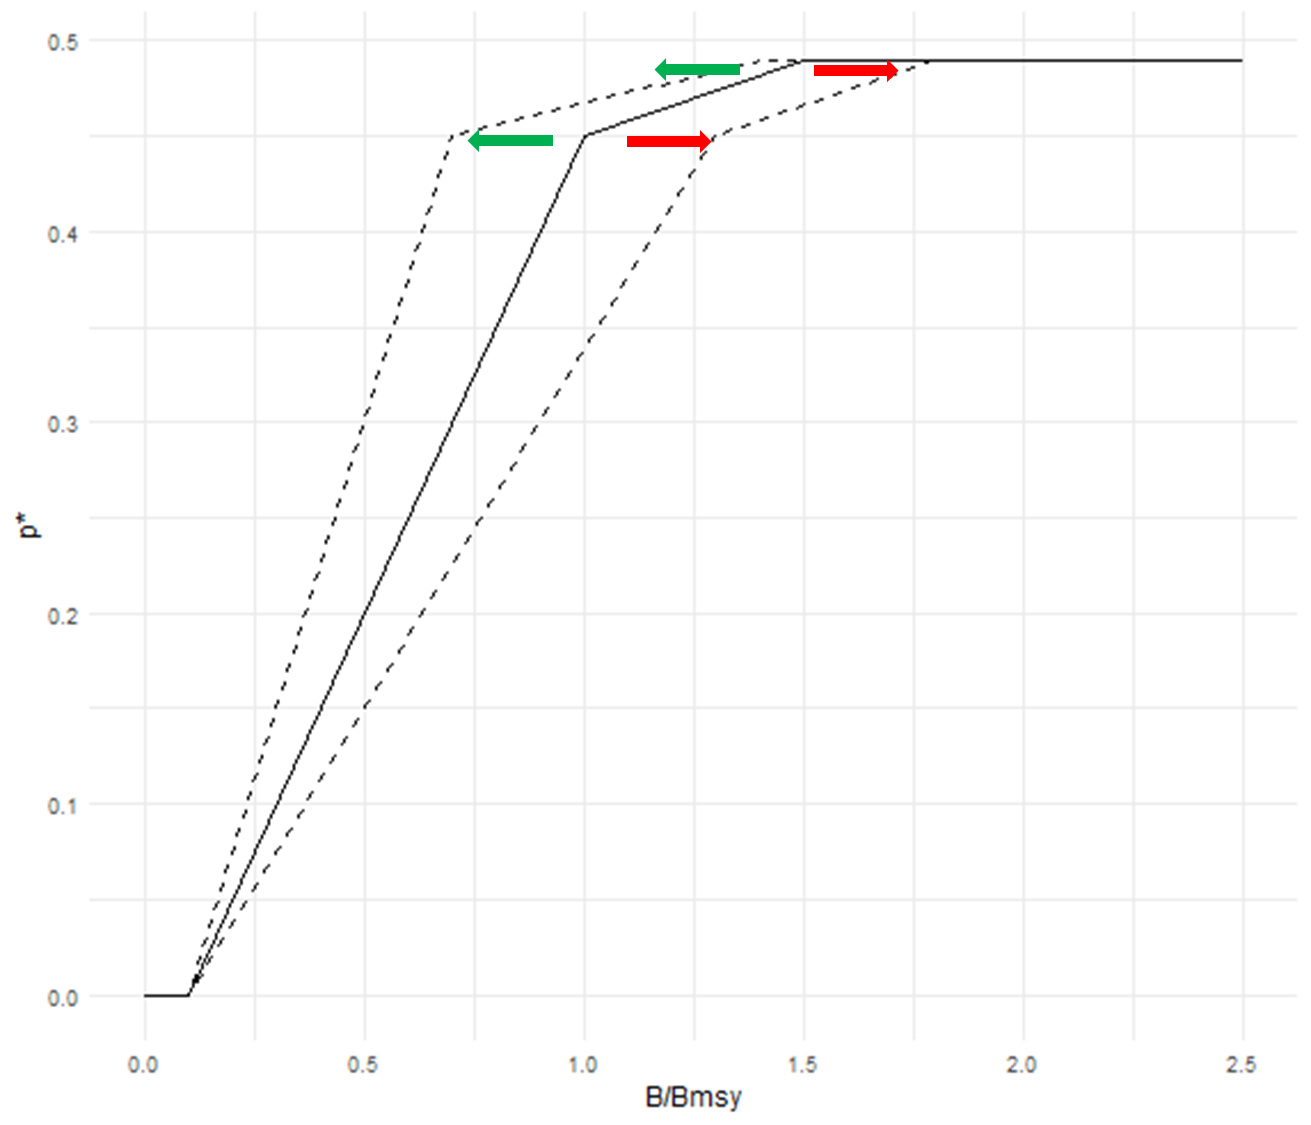
\includegraphics[width=0.8\linewidth]{../onepagers/RiskPolInds} 

}

\caption{Example indicator-based adjustments to risk policy, with increased risk tolerance indicated by green arrows and decreased risk tolerance indicated by red arrows.}\label{fig:newriskpol}
\end{figure}

\subsubsection{Information gaps}\label{information-gaps}

Ecosystem and Socioeconomic Profiles do not yet exist for the species originally used to evaluate the Risk Policy: summer flounder, scup, and butterfish.

\subsection{Catch/Quota Setting}\label{catchquota-setting}

Catch and Quota Setting is a multistep process involving decisions by the Northeast Regional Coordinating Committee (NRCC; including the Mid Atlantic and New England Councils, ASMFC, and NOAA's GARFO and NEFSC), assessment scientists, assessment peer reviewers, the Council's SSC, Monitoring Committees, and the Council. Information for each stock and fishery is reviewed and synthesized to determine catch and quota levels that meet management objectives.

\subsubsection{What information is used now?}\label{what-information-is-used-now-1}

There are 5 steps in the Catch/Quota setting process, described in general here and elaborated in 1-pagers for each step. We include the details for steps 4 and 5 here as these were the focus of the workshop presentation.

\textbf{1. Determine Assessment Priorities}

The NRCC prioritizes stocks for assessment based on management needs,
fishery importance, stock status and trend, ecosystem importance, assessment information, and stock
biology. Terms of Reference (ToRs) ensure the assessment process delivers consistent, management-relevant outputs.

\textbf{2. Conduct Assessment}

Assessment scientists assemble and analyze fishery dependent and independent data and develop models to synthesize the data and produce outputs meeting the assessment ToRs.

\textbf{3. Review Assessment}

Independent peer reviewers evaluate whether assessment ToRs are met, data is appropriate, and methods reflect best practices.

\textbf{4. Determine Acceptable Biological Catch (ABC)}

The SSC uses reviewed assessment outputs within a structured framework to determine ABC from assessment uncertainty based on input data, model diagnostics and performance, and ecosystem considerations.

The stock assessment gives current status and short term projections of overfishing limit (OFL) that may or may not already include ecosystem information. The SSC may discuss performance of short term projections or terminal year estimates in the assessment; ecosystem information can inform decisions about projections or terminal year estimates. The SSC may request new OFL estimates/projections from the assessment lead based on this discussion.

The SSC uses its \href{https://www.mafmc.org/s/Final-OFL-CV-guidance-document_06_24.pdf}{OFL CV process} to evaluate scientific uncertainty arising from data quality, model selection/identification, retrospective analysis, empirical comparisons, ecosystem factors, and recruitment stanzas. Ecosystem information can feed into:

\begin{itemize}
\tightlist
\item
  Ecosystem factors: \href{https://journals.plos.org/plosone/article?id=10.1371/journal.pone.0146756}{Climate Vulnerability Analysis} results are currently included for each stock, can include multiple other environmentally driven changes in the stock
\item
  Recruitment stanzas: links to environmental drivers can decrease recruitment uncertainty
\end{itemize}

Ecosystem information that is presented along with the assessment is easiest to use in the OFL CV determination, but nothing limits the SSC from using ecosystem information presented from other sources. The SSC has based decisions on published literature in the past.

The OFL CV is used along with the estimate of current stock status in the \href{http://www.mafmc.org/s/MAFMC-ABC-Control-Rule-White-Paper.pdf}{MAFMC ABC control rule} to determine the ABC that is recommended to the Council. The SSC often provides annually averaged constant ABC for a specified period (2-3 years) as well as annual ABC for each year at the request of the Council.

\textbf{5. Catch Limits, Targets, and Quotas}

The Council decides whether annually varying or averaged ABCs will be used in multiyear harvest specifications, then allocates the ABC to harvest sectors, if appropriate. Management uncertainty is determined and applied, then discards are estimated and subtracted to derive commercial quotas and recreational harvest limits.

\emph{Details vary by FMP} but in general:

The Council decides whether to use constant ABC or annual ABC for the specification years.

The ABC is split to recreational and commercial sector Annual Catch Limit (ACL), if applicable: the percentage is defined in the FMP, and requires an amendment or framework to change.

The Monitoring Committee recommends a management uncertainty buffer to determine the Annual Catch Target (ACT) for each sector.

The Monitoring Committee projects sector specific discards and subtracts them from each sector's ACT to determine the total allowable landings limit, or Recreational Harvest Limit (RHL) and the commercial quota, depending on the FMP.

For some species, the commercial quota is allocated to states or seasons as specified in FMPs. These allocations require an amendment or framework to change.

\subsubsection{Information sources for indicators}\label{information-sources-for-indicators}

There are many potential sources for indicator use in the Catch/Quota setting process. Indicators are already used in Steps 1 and 2.

As noted above, existing \href{https://www.fisheries.noaa.gov/new-england-mid-atlantic/ecosystems/ecosystem-and-socioeconomic-profile-development-and-reports}{Ecosystem and Socioeconomic Profiles} conceptual models and indicators for MAFMC stocks include:

\begin{itemize}
\tightlist
\item
  Black Sea Bass
\item
  Bluefish
\item
  Golden Tilefish
\item
  Longfin squid
\item
  Shortfin squid
\end{itemize}

\href{https://www.fisheries.noaa.gov/new-england-mid-atlantic/ecosystems/state-ecosystem-reports-northeast-us-shelf}{State of the Ecosystem} and \href{https://www.mafmc.org/s/2_MAB_RiskAssess_2024.pdf}{EAFM Risk Assessment} indicators

The fish and invertebrate \href{https://journals.plos.org/plosone/article?id=10.1371/journal.pone.0146756}{Climate Vulnerability Analysis} sensitivity, exposure and vulnerability rankings

Multiple Essential Fish Habitat sources:

\begin{itemize}
\tightlist
\item
  \href{https://www.fisheries.noaa.gov/resource/map/essential-fish-habitat-mapper}{EFH Habitat Mapper}
\item
  \href{https://nrha.shinyapps.io/dataexplorer/}{NRHA Data Explorer}
\item
  \href{https://fishmaps.shinyapps.io/FishingEffectsDatabase/}{Fishing Gear Effects Database}
\end{itemize}

And many other potential sources:

\begin{itemize}
\tightlist
\item
  \href{https://www.fisheries.noaa.gov/inport/item/22549}{NEFSC Surveys}
\item
  \href{https://fwdp.shinyapps.io/tm2020/}{NEFSC Food Habits}
\item
  \href{https://www.vims.edu/research/units/programs/multispecies_fisheries_research/neamap/}{NEAMAP Survey and Food Habits}
\item
  \href{https://www.fisheries.noaa.gov/inport/item/27317}{Study Fleet} and other Cooperative Research Programs
\item
  \href{https://www.fisheries.noaa.gov/new-england-mid-atlantic/commercial-fishing/quota-monitoring-greater-atlantic-region}{GARFO Catch and Monitoring System}
\item
  \href{https://safis.accsp.org/accsp_prod/f?p=1490:1:6442641492940:::::}{Atlantic Coastal Cooperative Statistics Program}
\item
  \href{https://www.fisheries.noaa.gov/recreational-fishing-data/introduction-marine-recreational-information-program-data}{Marine Recreational Information Program}
\item
  \href{https://data.marine.copernicus.eu/product/GLOBAL_MULTIYEAR_PHY_001_030/description}{GLORYS ocean reanalysis}
\end{itemize}

\subsubsection{Potential Pathways}\label{potential-pathways-1}

\begin{itemize}
\tightlist
\item
  Ecosystem information can enter at some portion of steps 1, 2, 4, and 5. These pathways for steps 4 and 5 are detailed below, because these steps are under full Council control.
\item
  The Council could also recommend additional assessment or review ToRs in steps 1 and 3.
\end{itemize}

\paragraph{ABC Setting}\label{abc-setting}

\begin{itemize}
\tightlist
\item
  Refine OFL CV criteria for considering integrated ecosystem conditions
\item
  Develop criteria for considering ecosystem impacts in short term projections
\item
  Systematic translation of stock specific indicators into risk criteria as in the Pacific could simplify OFL CV discussions (Table \ref{tab:pacrisk} and see the \href{https://www.pcouncil.org/documents/2024/08/h-1-a-cciea-team-report-1-cciea-risk-table-report-on-fep-initiative-4.pdf/}{CCIEA Risk Table Report}).
\end{itemize}

\global\setlength{\Oldarrayrulewidth}{\arrayrulewidth}

\global\setlength{\Oldtabcolsep}{\tabcolsep}

\setlength{\tabcolsep}{2pt}

\renewcommand*{\arraystretch}{1.2}



\providecommand{\ascline}[3]{\noalign{\global\arrayrulewidth #1}\arrayrulecolor[HTML]{#2}\cline{#3}}

\begin{longtable}[c]{|p{1.00in}|p{4.00in}}

\caption{Pacific\ Pilot\ Risk\ Levels\ and\ Indicator\ Criteria}\label{tab:pacrisk}\\

\hhline{>{\arrayrulecolor[HTML]{666666}\global\arrayrulewidth=1.5pt}->{\arrayrulecolor[HTML]{666666}\global\arrayrulewidth=1.5pt}-}

\multicolumn{1}{>{\raggedright}m{\dimexpr 1in+0\tabcolsep}}{\textcolor[HTML]{000000}{\fontsize{9}{9}\selectfont{Risk\ Level}}} & \multicolumn{1}{>{\raggedright}m{\dimexpr 4in+0\tabcolsep}}{\textcolor[HTML]{000000}{\fontsize{9}{9}\selectfont{Ecosystem\ and\ Environmental\ Conditions}}} \\

\noalign{\global\arrayrulewidth 0pt}\arrayrulecolor[HTML]{000000}

\hhline{>{\arrayrulecolor[HTML]{666666}\global\arrayrulewidth=1.5pt}->{\arrayrulecolor[HTML]{666666}\global\arrayrulewidth=1.5pt}-}\endfirsthead \caption[]{Pacific\ Pilot\ Risk\ Levels\ and\ Indicator\ Criteria}\label{tab:pacrisk}\\

\hhline{>{\arrayrulecolor[HTML]{666666}\global\arrayrulewidth=1.5pt}->{\arrayrulecolor[HTML]{666666}\global\arrayrulewidth=1.5pt}-}

\multicolumn{1}{>{\raggedright}m{\dimexpr 1in+0\tabcolsep}}{\textcolor[HTML]{000000}{\fontsize{9}{9}\selectfont{Risk\ Level}}} & \multicolumn{1}{>{\raggedright}m{\dimexpr 4in+0\tabcolsep}}{\textcolor[HTML]{000000}{\fontsize{9}{9}\selectfont{Ecosystem\ and\ Environmental\ Conditions}}} \\

\noalign{\global\arrayrulewidth 0pt}\arrayrulecolor[HTML]{000000}

\hhline{>{\arrayrulecolor[HTML]{666666}\global\arrayrulewidth=1.5pt}->{\arrayrulecolor[HTML]{666666}\global\arrayrulewidth=1.5pt}-}\endhead



\multicolumn{1}{>{\cellcolor[HTML]{00FF00}\raggedright}m{\dimexpr 1in+0\tabcolsep}}{\textcolor[HTML]{000000}{\fontsize{9}{9}\selectfont{Level\ 1:\ Favorable}}} & \multicolumn{1}{>{\cellcolor[HTML]{00FF00}\raggedright}m{\dimexpr 4in+0\tabcolsep}}{\textcolor[HTML]{000000}{\fontsize{9}{9}\selectfont{Indicators\ not\ used\ in\ the\ stock\ assessment\ show\ medium\ to\ high\ level\ of\ agreement\ and\ moderate\ to\ strong\ evidence\ supporting\ high\ species\ productivity.}}} \\

\noalign{\global\arrayrulewidth 0pt}\arrayrulecolor[HTML]{000000}





\multicolumn{1}{>{\cellcolor[HTML]{FFFFFF}\raggedright}m{\dimexpr 1in+0\tabcolsep}}{\textcolor[HTML]{000000}{\fontsize{9}{9}\selectfont{Level\ 2:\ Neutral}}} & \multicolumn{1}{>{\cellcolor[HTML]{FFFFFF}\raggedright}m{\dimexpr 4in+0\tabcolsep}}{\textcolor[HTML]{000000}{\fontsize{9}{9}\selectfont{Majority\ of\ indicators\ show\ no\ notable\ trends\ and/or\ no\ apparent\ environmental\ and\ ecosystem\ concerns.}}} \\

\noalign{\global\arrayrulewidth 0pt}\arrayrulecolor[HTML]{000000}





\multicolumn{1}{>{\cellcolor[HTML]{FF0000}\raggedright}m{\dimexpr 1in+0\tabcolsep}}{\textcolor[HTML]{000000}{\fontsize{9}{9}\selectfont{Level\ 3:\ Unfavorable}}} & \multicolumn{1}{>{\cellcolor[HTML]{FF0000}\raggedright}m{\dimexpr 4in+0\tabcolsep}}{\textcolor[HTML]{000000}{\fontsize{9}{9}\selectfont{Majority\ of\ indicators\ show\ medium\ to\ high\ level\ of\ agreement\ and\ moderate\ to\ strong\ evidence\ supporting\ low\ species\ productivity}}} \\

\noalign{\global\arrayrulewidth 0pt}\arrayrulecolor[HTML]{000000}

\hhline{>{\arrayrulecolor[HTML]{666666}\global\arrayrulewidth=1.5pt}->{\arrayrulecolor[HTML]{666666}\global\arrayrulewidth=1.5pt}-}



\end{longtable}



\arrayrulecolor[HTML]{000000}

\global\setlength{\arrayrulewidth}{\Oldarrayrulewidth}

\global\setlength{\tabcolsep}{\Oldtabcolsep}

\renewcommand*{\arraystretch}{1}

\paragraph{Catch Limits, Targets, and Quotas}\label{catch-limits-targets-and-quotas}

Management uncertainty buffer estimation could include ecosystem information such as projected stock productivity and distribution. \href{https://www.fisheries.noaa.gov/new-england-mid-atlantic/ecosystems/ecosystem-and-socioeconomic-profile-development-and-reports}{Ecosystem and Socioeconomic Profiles} conceptual models and indicators for MAFMC stocks, the fish and invertebrate \href{https://journals.plos.org/plosone/article?id=10.1371/journal.pone.0146756}{Climate Vulnerability Analysis} sensitivity, exposure and vulnerability rankings, \href{https://www.fisheries.noaa.gov/new-england-mid-atlantic/ecosystems/state-ecosystem-reports-northeast-us-shelf}{State of the Ecosystem} and \href{https://www.mafmc.org/s/2_MAB_RiskAssess_2024.pdf}{Risk Assessment} indicators could be applied here.

Discard estimation/projection could include similar ecosystem information as above on projected stock productivity and distribution, and also consider habitat conditions leading to different product quality or discard survival based on multiple Essential Fish Habitat sources such as \href{https://www.fisheries.noaa.gov/resource/map/essential-fish-habitat-mapper}{EFH Habitat Mapper} or \href{https://nrha.shinyapps.io/dataexplorer/}{NRHA Data Explorer} combined with projected habitat conditions from \href{https://psl.noaa.gov/cefi_portal/}{MOM6 regional ocean projections}.

If FMP amendments or frameworks are considered to alter allocations, \href{https://www.fisheries.noaa.gov/new-england-mid-atlantic/commercial-fishing/quota-monitoring-greater-atlantic-region}{GARFO Catch and Monitoring System}, \href{https://safis.accsp.org/accsp_prod/f?p=1490:1:6442641492940:::::}{Atlantic Coastal Cooperative Statistics Program}, and \href{https://www.fisheries.noaa.gov/recreational-fishing-data/introduction-marine-recreational-information-program-data}{Marine Recreational Information Program} information along with
SOE or ESP economic and social indicators could inform these decisions.

\subsubsection{Information gaps}\label{information-gaps-1}

Ecosystem and Socioeconomic Profiles evaluate and select stock specific ecosystem and socioeconomic indicators that can be useful across many steps of the Catch/Quota setting process; these are currently unavailable for summer flounder, scup, Atlantic mackerel, butterfish, surfclam, ocean quahog, blueline tilefish, spiny dogfish, and monkfish.

\section{Workshop Discussion Summary}\label{workshop-discussion-summary}

Discussions made up the majority of the workshop. All discussions were conducted in plenary with all participants. Each discussion had a discussion facilitator from the project team and multiple note takers. At the end of the discussions, a project team lead summarized the main points. Notes from all discussions were reviewed and combined into this summary.

\subsection{Discussion 1: Relative merits of developing indicators for each priority decision}\label{discussion-1-relative-merits-of-developing-indicators-for-each-priority-decision}

\begin{enumerate}
\def\labelenumi{\arabic{enumi}.}
\tightlist
\item
  Risk policy and catch/quota setting were confirmed as the two priority decisions, with risk policy ranking highest. Spatial management was set aside for potential future exploration.\\
\item
  Participants emphasized the importance of avoiding ``double-dipping'' -- ensuring ecosystem indicators aren't applied redundantly at multiple steps in the management process where they are already explicitly or implicitly incorporated.\\
\item
  Participants stressed the importance of clear communication and transparent documentation of where and how ecosystem considerations enter the process. They also flagged data timing as a practical concern, noting that indicators need to be available when decisions are actually being made.\\
\item
  Socioeconomic indicators were identified as a promising area for development, particularly for risk policy, given that the current framework relies almost exclusively on biological indicators.
\end{enumerate}

\subsection{Discussion 2: Identify desirable and undesirable states for management outcomes}\label{discussion-2-identify-desirable-and-undesirable-states-for-management-outcomes}

\begin{enumerate}
\def\labelenumi{\arabic{enumi}.}
\tightlist
\item
  Participants favored defining desirable states in directional or relative terms (e.g., landings above a minimum threshold) rather than as fixed point targets.\\
\item
  The risk policy's existing simplicity was viewed as a strength worth preserving; however, past instances where the policy was suspended (driven by socioeconomic conditions) were identified as opportunities to formally embed additional indicator types.\\
\item
  Stability in management measures was raised as a desirable objective, with the idea that well-chosen indicators could reduce large year-to-year swings. However, adding indicators also risks increasing complexity.\\
\item
  There was interest in reframing desirable outcomes as operating within a complex of interconnected indicators rather than as single targets. For example, ``maintaining stability while still allowing fishing opportunities.''\\
\item
  It was noted that a particularly undesirable outcome would result in cascading, unanticipated effects that force managers into reactive correction rather than proactive management.
\end{enumerate}

\subsection{Discussion 3: Discuss potential indicator targets or thresholds tied to states above}\label{discussion-3-discuss-potential-indicator-targets-or-thresholds-tied-to-states-above}

\begin{enumerate}
\def\labelenumi{\arabic{enumi}.}
\tightlist
\item
  Participants broadly agreed that thresholds should be expressed as ranges rather than fixed points, with a historical baseline period used as a reference while allowing for adaptability as system conditions change.\\
\item
  There was strong agreement that percent-change constraints on management measures (e.g., year-to-year quota changes) should apply for recreational and commercial fisheries if implemented, and that stock status should factor into what level of change is considered acceptable.\\
\item
  Uncertainty quantification was highlighted as an important issue, with concern that the current SSC process sometimes defaults to conservative CV values regardless of data quality. Participants highlighted the need for more explicit tracking of both sources of certainty and uncertainty.\\
\item
  The concept of ``surveillance indicators'' was discussed as a potential framework, referring to pre-defined flags that trigger extra scrutiny when conditions fall outside an acceptable or recently/historically observed range, rather than requiring a rigid management response.
\end{enumerate}

\section{Next Steps}\label{next-steps}

Approach: adjustment to current processes with indicators, not invention of new processes

\subsection{Risk Policy: general scope and keep it simple}\label{risk-policy-general-scope-and-keep-it-simple}

\textbf{Guiding question:} What is the range of acceptable tradeoffs between social/economic considerations and stock status at a given level of overfishing risk? Can the use of multiple indicators increase stability in advice?

\textbf{Initial needs}

\begin{itemize}
\tightlist
\item
  Documentation for each time Council has suspended the risk policy.
\item
  Request code from Weidenmann for 2019 risk policy MSE.
\end{itemize}

\textbf{Focus on social and economic indicators}

\begin{itemize}
\tightlist
\item
  Integrate concerns that caused risk policy suspension.
\item
  Review current SOE, Risk Assessment, SSB Performance.
\item
  Draw dataset from Fishery Performance reports.
\end{itemize}

\subsection{Catch/Quota setting: species scope and avoid double counting}\label{catchquota-setting-species-scope-and-avoid-double-counting}

\textbf{Focus on indicators for Steps 4 and 5: under Council control}

\begin{itemize}
\tightlist
\item
  List indicators/processes currently used steps 1-3 to avoid double counting, but don't suggest new indicators in these steps.
\item
  NRCC and NEFSC already have processes to use indicators for prioritization and assessment, respectively.
\end{itemize}

It was noted that making Steps 4 and 5 work with indicators but without assessments is a potentially important future issue that this project could address. The project team will evaluate the feasibility of developing options for indicator-based decision making in the absence of stock assessments and report back at the next workshop.

\textbf{Clarifications needed}

The project team requested clarification during the workshop regarding these questions.

\begin{itemize}
\tightlist
\item
  Step 5: evaluate indicators for both occasional strategic and routine tactical? Are we tackling allocation or not?
\item
  Which focal species: Black sea bass, summer flounder, squid, a combination?
\end{itemize}

The scope for use of indicators in this process was not limited by the workshop participants, and species selection was narrowed to the group above but no single species was selected. The project team will consider routine/tactical committee decisions and strategic FMP decisions for indicator development across up to two contrasting species, and bring a range of options back at the next workshop.

The project team will also consider whether it is feasible to evaluate results from indicator use across both the risk policy and a selected species catch/quota setting process and present that scenario at the next workshop.

\subsection{Planned Analyses through 2026}\label{planned-analyses-through-2026}

Quantitative indicator development and testing will proceed for Risk Policy and Catch/Quota Setting (ABC and ACL/ACT/Quotas, Steps 4 and 5). Indicators are related to management decisions using targets (ideal states) and thresholds (transitions to undesirable states; {[}\citeproc{ref-link_translating_2005}{1},\citeproc{ref-hiddink_setting_2023}{2}{]}). Literature review for theoretical ecosystem targets and thresholds associated with the Council's priority decisions will begin.

Indicator data sources will be evaluated to ensure timely updates of indicators, and code will be developed to ensure future data updates are done consistently over time, similar to the process used for the NEFSC ecodata indicator dataset {[}\citeproc{ref-bastille_improving_2021}{3}{]}. some new indicator datasets may need to be acquired or synthesized from multiple sources. Some model development (e.g.~updates to existing spatial, population dynamics, ecosystem, and or economic models) may also be needed to facilitate indicator development and testing. Once sufficient indicator data are available, testing for empirical indicator thresholds {[}\citeproc{ref-large_quantifying_2015}{4}--\citeproc{ref-tam_comparing_2017}{7}{]} will begin. Desired states identified by the Council and any potentially beneficial or problematic states emergent from the analysis will be documented for each priority indicator. The development of priority indicators and empirical testing of targets and thresholds will be done between April and December of 2026.

Once potential targets and thresholds are identified for each priority indicator, they will be simulation tested to evaluate indicator target and threshold performance under a range of environmental conditions {[}\citeproc{ref-fay_testing_2013}{8}{]}. Testing indicator performance within multispecies, socio-economic, or ecosystem models will facilitate holistic understanding of the behavior of management targets and thresholds beyond the intended decision {[}\citeproc{ref-samhouri_quantitative_2009}{9},\citeproc{ref-tam_better_2019}{10}{]}.

Beginning in Fall of 2026, the Project team and Project Oversight Team will collaboratively develop a list of potential indicator performance metrics for Council consideration. We will facilitate a second in-person Council workshop when sufficient indicator data and preliminary targets and thresholds are available for review, approximately mid-way through Phase 2 (December 2026).

\section{List of Appendices}\label{list-of-appendices}

\begin{enumerate}
\def\labelenumi{\arabic{enumi}.}
\tightlist
\item
  Workshop \href{https://www.mafmc.org/s/1_Final-Mini-Workshop-Agenda.pdf}{Agenda}
\item
  Workshop Attendees
\item
  Workshop Overview \href{https://www.mafmc.org/s/2_MiniWK_Overview.pdf}{1-pager}
\item
  Risk Policy \href{https://www.mafmc.org/s/3_MiniWK_RiskPolicy.pdf}{1-pager}
\item
  Catch/Quota Setting Overview \href{https://www.mafmc.org/s/4_MiniWK_CatchQuotas.pdf}{1-pager}

  \begin{itemize}
  \tightlist
  \item
    Catch/Quota Setting Step 1: Prioritization \href{https://www.mafmc.org/s/4a_MiniWK_CatchQuotas_1_Prioritize.pdf}{1-pager}
  \item
    Catch/Quota Setting Step 2: Assessment \href{https://www.mafmc.org/s/4b_MiniWK_CatchQuotas_2_Assess.pdf}{1-pager}
  \item
    Catch/Quota Setting Step 4: ABC \href{https://www.mafmc.org/s/4c_MiniWK_CatchQuotas_4_ABC.pdf}{1-pager}
  \item
    Catch/Quota Setting Step 5: ACL/ACT/Quotas \href{https://www.mafmc.org/s/4d_MiniWK_CatchQuotas_5_ACLACTQuota.pdf}{1-pager}
  \end{itemize}
\item
  Measures Setting \href{https://www.mafmc.org/s/5_MiniWK_MeasuresSetting.pdf}{1-pager}
\item
  Spatial Measures \href{https://www.mafmc.org/s/6_MiniWK_SpatialMeasures.pdf}{1-pager}
\item
  Workshop Summary \href{}{1-pager}
\end{enumerate}

\section*{References}\label{references}
\addcontentsline{toc}{section}{References}

\phantomsection\label{refs}
\begin{CSLReferences}{0}{1}
\bibitem[\citeproctext]{ref-link_translating_2005}
\CSLLeftMargin{1. }%
\CSLRightInline{Link JS. Translating ecosystem indicators into decision criteria. ICES Journal of Marine Science. 2005;62: 569--576. doi:\href{https://doi.org/10.1016/j.icesjms.2004.12.015}{10.1016/j.icesjms.2004.12.015}}

\bibitem[\citeproctext]{ref-hiddink_setting_2023}
\CSLLeftMargin{2. }%
\CSLRightInline{Hiddink JG, Valanko S, Delargy AJ, Denderen PD van. Setting thresholds for good ecosystem state in marine seabed systems and beyond. ICES Journal of Marine Science. 2023;80: 698--709. doi:\href{https://doi.org/10.1093/icesjms/fsad035}{10.1093/icesjms/fsad035}}

\bibitem[\citeproctext]{ref-bastille_improving_2021}
\CSLLeftMargin{3. }%
\CSLRightInline{Bastille K, Hardison S, deWitt L, Brown J, Samhouri J, Gaichas S, et al. Improving the {IEA} {Approach} {Using} {Principles} of {Open} {Data} {Science}. Coastal Management. 2021;49: 72--89. doi:\href{https://doi.org/10.1080/08920753.2021.1846155}{10.1080/08920753.2021.1846155}}

\bibitem[\citeproctext]{ref-large_quantifying_2015}
\CSLLeftMargin{4. }%
\CSLRightInline{Large SI, Fay G, Friedland KD, Link JS. Quantifying {Patterns} of {Change} in {Marine} {Ecosystem} {Response} to {Multiple} {Pressures}:~e0119922. PLoS One. 2015;10. doi:\url{http://dx.doi.org/10.1371/journal.pone.0119922}}

\bibitem[\citeproctext]{ref-large_defining_2013}
\CSLLeftMargin{5. }%
\CSLRightInline{Large SI, Fay G, Friedland KD, Link JS. Defining trends and thresholds in responses of ecological indicators to fishing and environmental pressures. ICES Journal of Marine Science: Journal du Conseil. 2013;70: 755--767. doi:\href{https://doi.org/10.1093/icesjms/fst067}{10.1093/icesjms/fst067}}

\bibitem[\citeproctext]{ref-samhouri_defining_2017}
\CSLLeftMargin{6. }%
\CSLRightInline{Samhouri JF, Andrews KS, Fay G, Harvey CJ, Hazen EL, Hennessey SM, et al. Defining ecosystem thresholds for human activities and environmental pressures in the {California} {Current}. Ecosphere. 2017;8: e01860. doi:\href{https://doi.org/10.1002/ecs2.1860}{10.1002/ecs2.1860}}

\bibitem[\citeproctext]{ref-tam_comparing_2017}
\CSLLeftMargin{7. }%
\CSLRightInline{Tam JC, Link JS, Large SI, Andrews K, Friedland KD, Gove J, et al. Comparing {Apples} to {Oranges}: {Common} {Trends} and {Thresholds} in {Anthropogenic} and {Environmental} {Pressures} across {Multiple} {Marine} {Ecosystems}. Frontiers in Marine Science. 2017;4. doi:\href{https://doi.org/10.3389/fmars.2017.00282}{10.3389/fmars.2017.00282}}

\bibitem[\citeproctext]{ref-fay_testing_2013}
\CSLLeftMargin{8. }%
\CSLRightInline{Fay G, Large SI, Link JS, Gamble RJ. Testing systemic fishing responses with ecosystem indicators. Ecological Modelling. 2013;265: 45--55. doi:\href{https://doi.org/10.1016/j.ecolmodel.2013.05.016}{10.1016/j.ecolmodel.2013.05.016}}

\bibitem[\citeproctext]{ref-samhouri_quantitative_2009}
\CSLLeftMargin{9. }%
\CSLRightInline{Samhouri JF, Levin PS, Harvey CJ. Quantitative {Evaluation} of {Marine} {Ecosystem} {Indicator} {Performance} {Using} {Food} {Web} {Models}. Ecosystems. 2009;12: 1283--1298. doi:\href{https://doi.org/10.1007/s10021-009-9286-9}{10.1007/s10021-009-9286-9}}

\bibitem[\citeproctext]{ref-tam_better_2019}
\CSLLeftMargin{10. }%
\CSLRightInline{Tam JC, Fay G, Link JS. Better {Together}: {The} {Uses} of {Ecological} and {Socio}-{Economic} {Indicators} {With} {End}-to-{End} {Models} in {Marine} {Ecosystem} {Based} {Management}. Frontiers in Marine Science. 2019;6. doi:\href{https://doi.org/10.3389/fmars.2019.00560}{10.3389/fmars.2019.00560}}

\end{CSLReferences}

\end{document}
